\documentclass[a4paper, 12pt]{article}
\usepackage[left=3cm,right=3cm,top=3cm,bottom=2cm]{geometry}
\usepackage{float}

\usepackage{preamble}

\begin{document}

	\thispagestyle{empty}

	\begin{center}
		\sc\bf
		Proposta de Trabalho Prático de\\
		Tópicos Especiais de Aprendizado de Máquina-TEAM\\
		Aprendizagem Profunda e por Reforço

		Daniel A. Torquato
	\end{center}

	Baseado no problema \emph{Hide and Seek} (Esconde-esconde) este trabalho
	busca uma resolução através dos métodos de Reinforcement Learning e
	Adversarial Network.

	\subsubsection*{Definição do Problema}

	Dado um mapa representação um determinado ambiente e dois agentes, um
	rastreador e outro fugitivo, o rastreador deve encontrar o fugitivo e
	retornar a um ponto de referência, por outro lado, o fugitivo deve chegar no
	ponto de referência antes que o rastreador alcance seu objetivo.


	\subsubsection*{Representação do problema}

	Será utilizado um simulador de 2d para representar os possíveis ambientes
	bem como os agentes. O ambiente pode será representado por uma imagem onde
	os pixel preto representam obstáculos intransponíveis, já os agentes será
	representados por triângulos coloridos. Cada agente possuirá uma câmera e um
	laser, que poderão ter suas resoluções alteradas, sendo estes mais 
	parâmetros a serem sintonizados.

	%\begin{figure}[H]
	%	\centering
	%	\includegraphics[width=2.5cm]{fig/robot4.png}
	%	\includegraphics[width=2.5cm]{fig/robot1.png}
		%\includegraphics[width=2.5cm]{fig/robot2.png}
	%	\includegraphics[width=5cm]{fig/robot3.png}
	%	\caption{Perfil dos agentes e Ambiente de simulação}
	%\end{figure}

	%Obs: O simulador utilizado tem um comunicação robusta com ROS (Robot
	%Operational System).


	\subsubsection*{Arquitetura e Método proposto}

	O método de aprendizado consiste na implementação do algoritmo A3C em cada
	agente do mesmo tipo (rastreador e fugitivo), por sua vez os agentes de tipo
	diferente serão treinados adversarialmente. Alguns parâmetros são comuns aos
	dois tipos de agentes, que seria aprender quais locais são bons para se
	esconder no mapa atual, assim a rede proposta possuirá uma parte comum. A
	recompensa será dada apenas quando os agentes alcançarem seus objetivos,
	porém para acelerar a aprendizagem é possível que algumas recompensas
	auxiliares sejam utilizadas, por exemplo para aprender encontrar o ponto de
	referência pode ser dado uma recompensa específica, assim como para
	identificar os oponentes ou para não colidir com a parede. A
	figura~\ref{fig1} mostra a arquitetura da rede neural proposta para o
	problema.

	\begin{figure}[H]
		\centering
	%	\includegraphics[width=2.5cm]{fig/robot4.png}
	%	\includegraphics[width=2.5cm]{fig/robot1.png}
		%\includegraphics[width=2.5cm]{fig/robot2.png}
		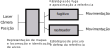
\includegraphics[width=10cm]{fig/rede.png}
		\caption{Rede aprendida pelos agentes}\label{fig1}
	\end{figure}

	Ao final se espera que os agentes tenha aprendido seus objetivos e formas de
	alcança-los de modo eficiente.



\end{document}
